%%%%%%%%%%%%%%%%%%%%%%%%%%%%%%%%%%%%%%%%%%%%%%%%%%%%%%%%%%%%%%%%%
% !TEX root = interimreport.tex

\clearpage
\chapter{PATH OF AN INSTRUCTION}\label{Ch4}
%%%%%%%%%%%%%%%%%%%%%%%%%%%%%%%%%%%%%%%%%%%%%%%%%%%%%%%%%%%%%%%%%
In this chapter, the path of an instruction will be demonstrated and the corresponding DAG input of the most critical phases of SelectionDAG will be shown. We selected the input program as a function that performs multiplication and addition. This was our litmus test code used while adding MLA (Multiply and Add) instruction to the LLVM backend with TableGen. We explained our addition of MLA instruction thoroughly in Section \ref{sec:MLA_add_section}. 

\begin{lstlisting}[language=C, caption=madd.c program]
int a,b,c;
void maddFunc() {
	a = 3;
	b = 103;
	
	c = 127;
	a = a * b +c;
}
\end{lstlisting}

\section{Clang AST}
You can see the Abstract Syntax Tree (AST) produced by Clang in Figure \ref{fig:clang_ast}. The AST consists of an expression tree with three levels. At the highest level there is an expression tree of multiplication between variables 'a' and 'b'. This expression tree's result becomes an argument for another expression tree with the addition operator. The second argument at this addition subtree is the variable 'c'. The expression tree at the root has assignment as an operator. The first argument to this tree is 'a' and the second argument is the result of multiplication and addition. Figure \ref{fig:ast_mla} shows the entire expression tree with the operations multiply and add. 

\begin{figure}
    \centering
    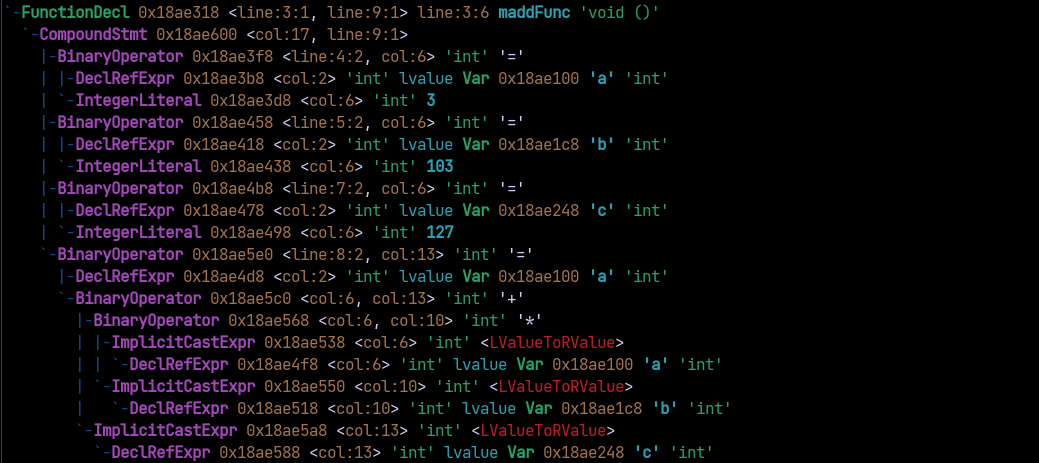
\includegraphics[width=\textwidth]{path_instruction/madd_clang_ast_cropped.png}
    \caption{AST generated by Clang}
    \label{fig:clang_ast}
\end{figure}
\begin{figure}
    \centering
\begin{tikzpicture}

    \node {=} [sibling distance = 2.5cm]
    child {node {+}
    child {node {*}
    child {node {\bf a}}
    child {node {\bf b}}}
    child {node {\bf c}}}
    child {node {\bf a}};
\end{tikzpicture}
    \caption{AST of MLA operation}
    \label{fig:ast_mla}
\end{figure}
\section{LLVM IR}
Clang CodeGen produces LLVM IR with the AST as the input. Figure \ref{fig:llvm_ir} shows the produced LLVM IR. The optimized LLVM IR is the input to SelectionDAG to generate target-specific instructions.  
\par
\begin{figure}
    \centering
    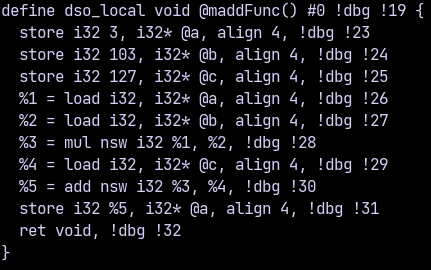
\includegraphics[width=0.6\textwidth]{path_instruction/madd_ll.png}
    \caption{LLVM IR file generated at the output of Clang}
    \label{fig:llvm_ir}
\end{figure}

\section{SelectionDAG}
 Input DAGs to SelectionDAG's passes will be demonstrated so on. The following phases will be demonstrated:
\begin{enumerate}
    \item First Optimization
    \item Legalization
    \item Second Optimization
    \item Instruction Selection
    \item Instruction Scheduling 
    \item Register Allocation
    \item Register sdsfsdfsdf

\end{enumerate}
\subsection{First Optimization Pass}
Figure \ref{fig:combine1} shows the DAG before the first optimization pass. It is the direct translation of LLVM IR to DAG form. After optimization, redundant nodes will be removed such as "Constant<0>" node.
\begin{figure}
    \centering
    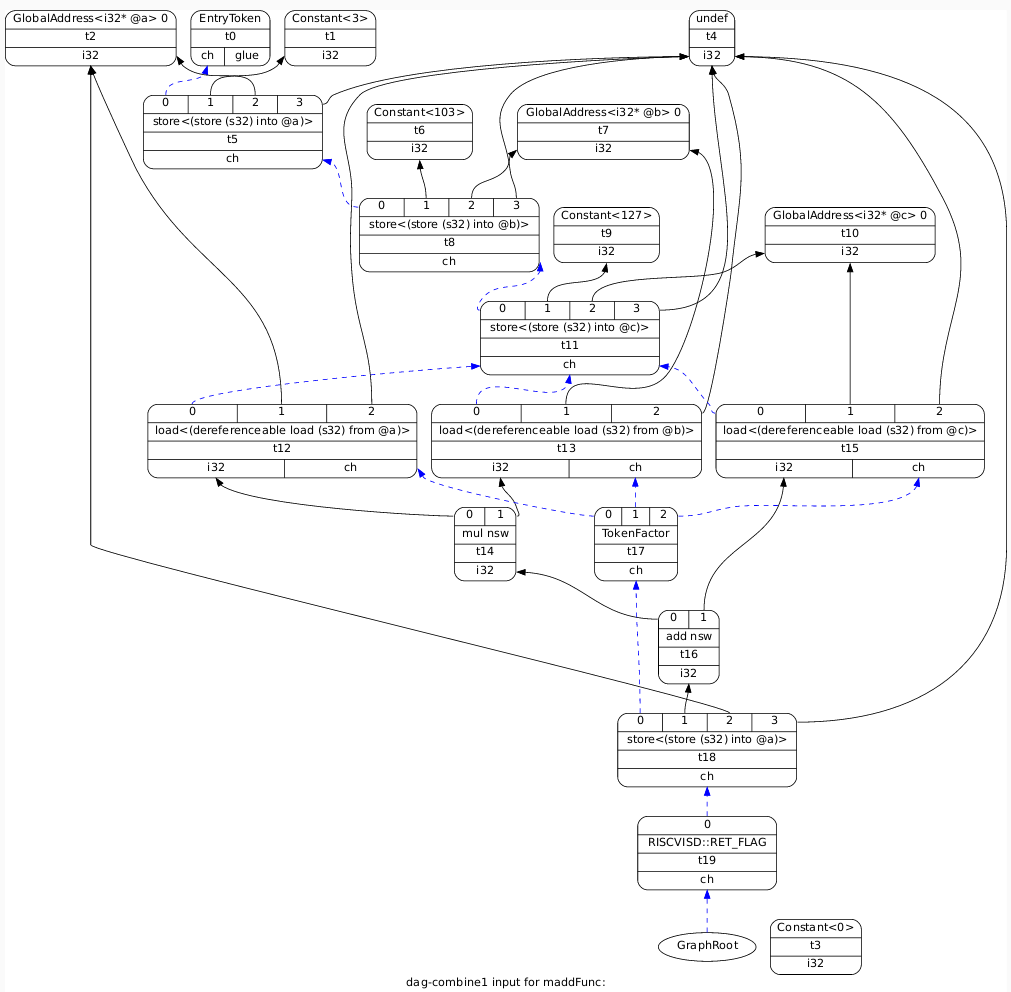
\includegraphics[width=0.9\textwidth]{path_instruction/madd_dag_combine1.png}
    \caption{DAG before first optimization pass}
    \label{fig:combine1}
\end{figure}

Figure \ref{fig:legalize} shows the DAG before legalization. The first optimization took place by removing nodes that do not contribute to the DAG. However, the instructions are not, in LLVM terms, "legal" as these general Machine Instructions do not map directly to every target's instructions.  

\subsection{Instruction Legalization}

\begin{figure}
    \centering
    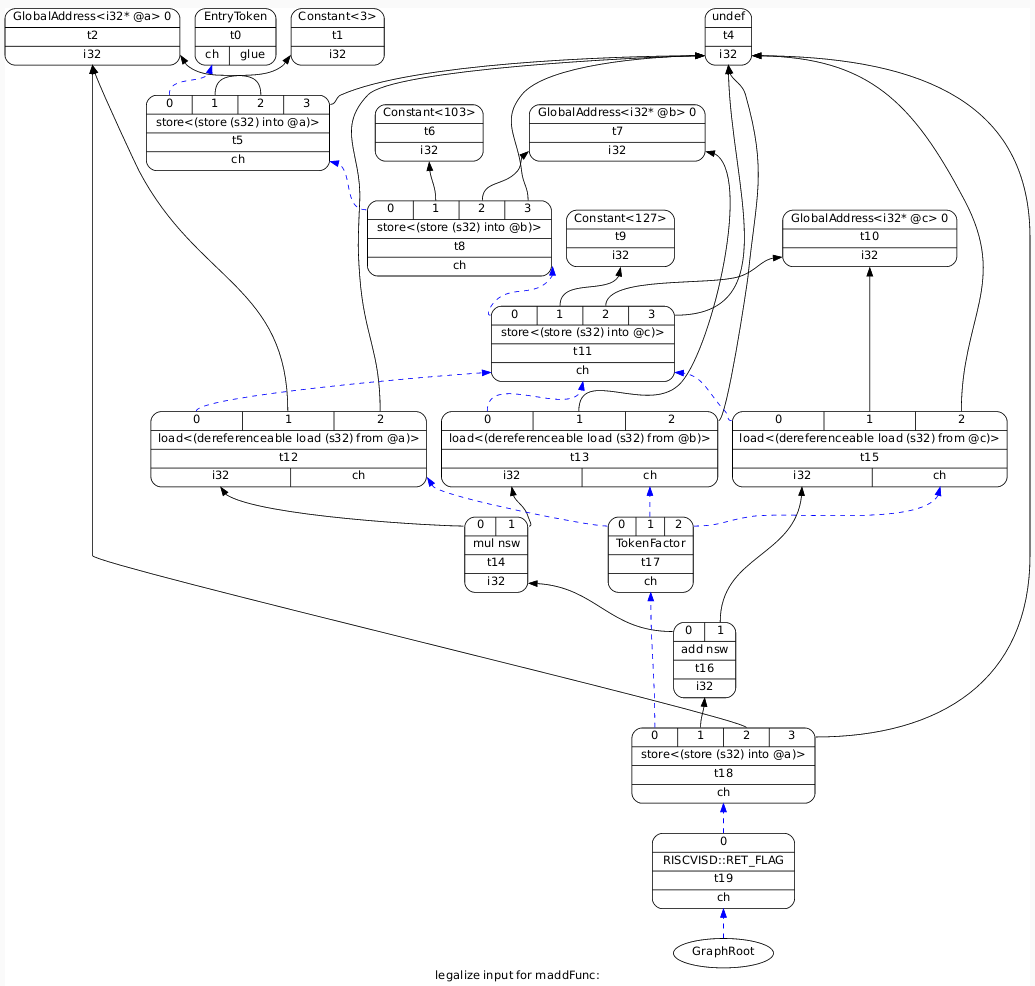
\includegraphics[width=0.9\textwidth]{path_instruction/madd_dag_legalize.png}
    \caption{DAG before Legalization}
    \label{fig:legalize}
\end{figure}

Figure \ref{fig:combine2} shows the DAG before the second optimization pass. The DAG is legalized by introducing RISCVISD::ADD\_LO and RISCVISD::HI nodes. These SelectionDAG nodes act as flags to give target-specific information to target-independent algorithms. These definitions are introduced at lib/Target/RISCV/RISCVISelLowering.h file \cite{riscvIselh}. It is the RISCV DAG lowering interface. 
\par
According to the interface file, RISCVISD::ADD\_LO is meant to add Lo 12 bits from an address and to be replaced by ADDI (Add Immediate) at Instruction Selection. Similarly, RISCVISD::HI is meant to get Hi 20 bits from an address and to be replaced by LUI (Load Upper Immediate). With a legalized DAG the second optimization pass begins.
\subsection{Second Optimization Pass}
\begin{figure}
    \centering
    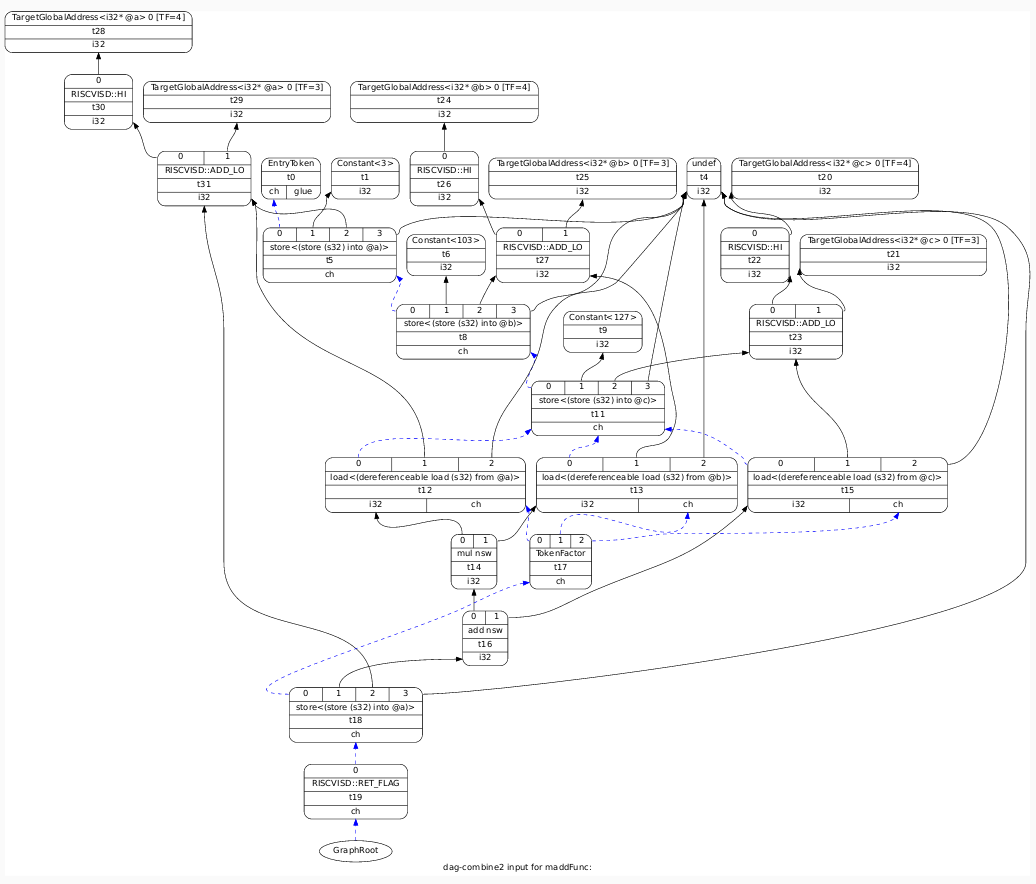
\includegraphics[width=0.9\textwidth]{path_instruction/madd_dag_combine2.png}
    \caption{DAG before the second optimization}
    \label{fig:combine2}
\end{figure}

Figure \ref{fig:isel} shows the DAG before the Instruction Selection phase. Comparison of Figure \ref{fig:combine2} and \ref{fig:isel} indicates that the second optimization did not change the DAG. This may be due to the reason that the subgraphs including the legalized nodes are not complex enough as the input C code is minimal.
\par
The DAG nodes up until Instruction Selection are instances of SDNode class which are target-independent nodes.
\begin{figure}
    \centering
    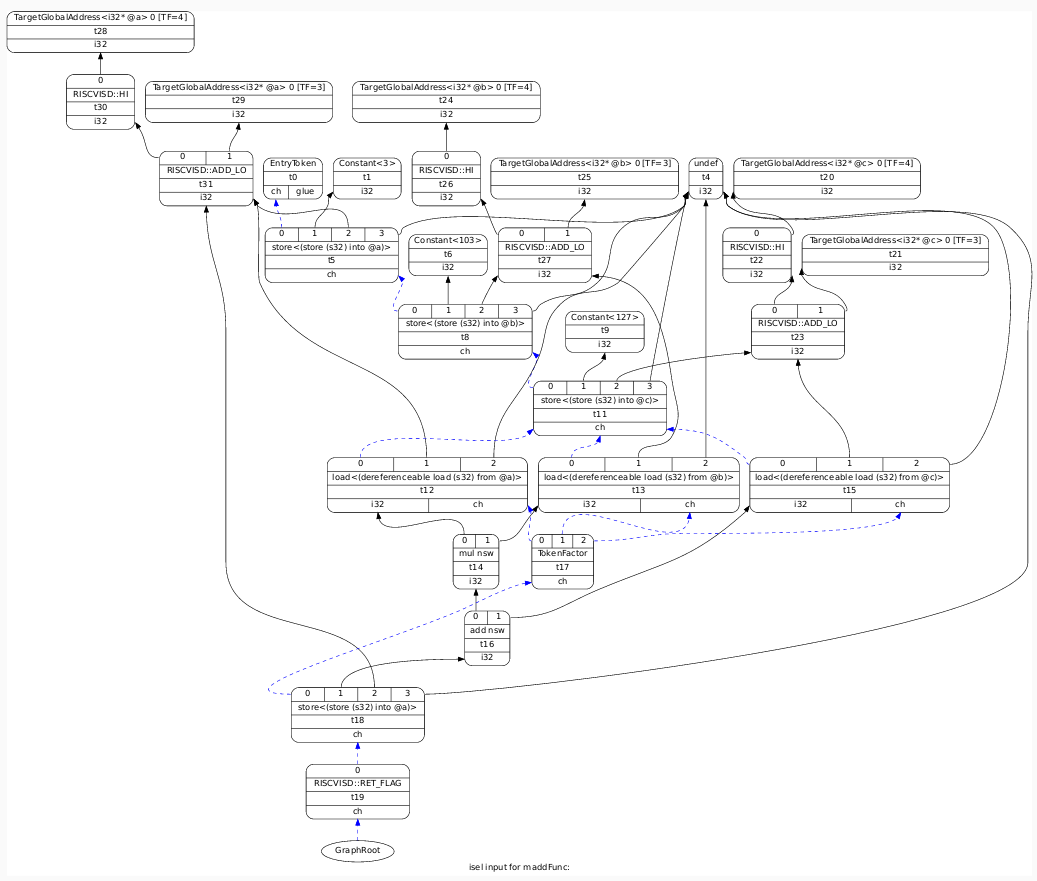
\includegraphics[width=0.9\textwidth]{path_instruction/madd_dag_isel.png}
    \caption{DAG before Instruction Selection}
    \label{fig:isel}
\end{figure}

\subsection{Instruction Selection}
Figure \ref{fig:dag_sched} shows the DAG before the Instruction Scheduling phase. You can see that the instructions are selected according to the RISC-V target. SDNode class nodes are replaced by MachineSDNode class nodes which are target-specific.
\par
RISCVISD nodes are replaced by their counterparts. The general Load and Store instructions are replaced by their type-aware corresponding LW (Load Word) and SW (Store Word) instructions. Most importantly the MLA instruction is selected replacing the subgraph of 'mul' and 'add' LLVM instructions. 
\par
We defined MLA instruction's DAG pattern as in the subgraph. The instruction selection phase took it as a reference, detected the pattern inside the global DAG and used it to place the MLA node. The addition process is explained more thoroughly in Section \ref{MLA_add_section}.

\begin{figure}
    \centering
    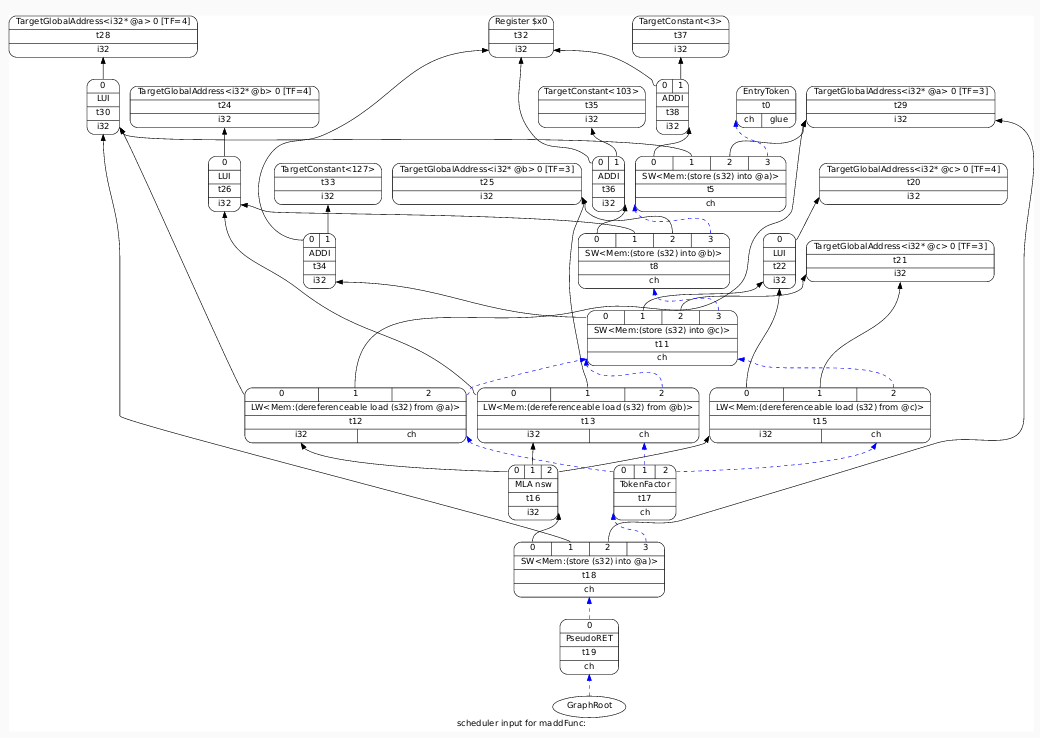
\includegraphics[width=0.9\textwidth]{path_instruction/madd_dag_sched.png}
    \caption{DAG before Instruction Scheduling}
    \label{fig:dag_sched}
\end{figure}

\subsection{Instruction Scheduling}
The DAG is transformed into a target-specific DAG with the result of legalization and selection phases. However, to generate a linear byte sequence, the DAG must be flattened. The instruction scheduling phase gets the DAG and linearises it according to the dependency graph of nodes. The scheduling dependency can be seen in Figure \ref{fig:sunit}.

\begin{figure}
    \centering
    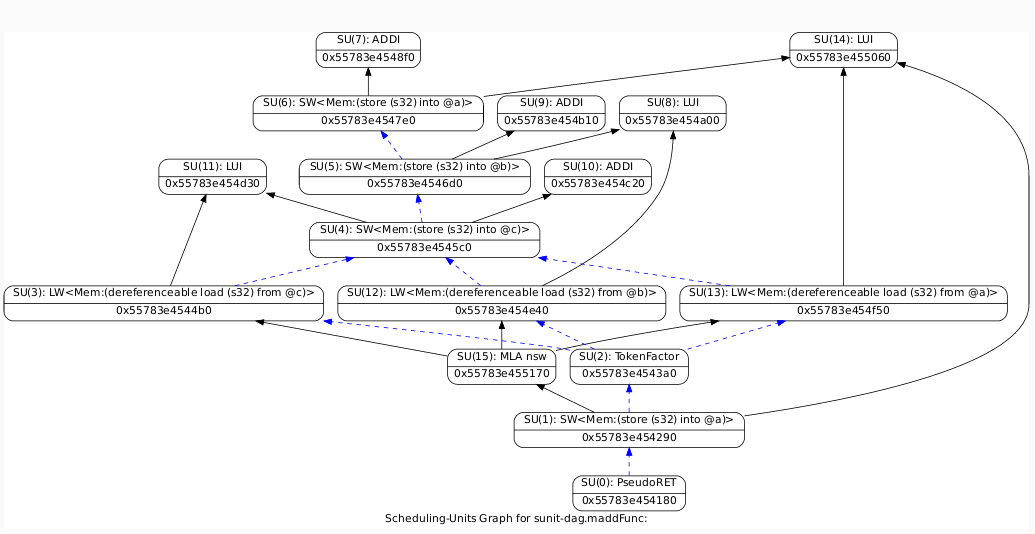
\includegraphics[width=0.9\textwidth]{path_instruction/madd_dag_sunit.png}
    \caption{Scheduling Dependency Graph}
    \label{fig:sunit}
\end{figure}


\subsection{Machine Instruction in SSA Form}
The generated Machine Instruction as a result of scheduling is shown in Figure \ref{fig:mc_inst}. Because register allocation is not yet performed, the instructions are in SSA (Static Single Assignment) form. In SSA form, virtual registers are considered to be infinite unless some specific registers have to be used. In this case, '\$x0' is mentioned with ADDI instructions as they are hardwired zero in RISC-V. 

\begin{figure}
    \centering
    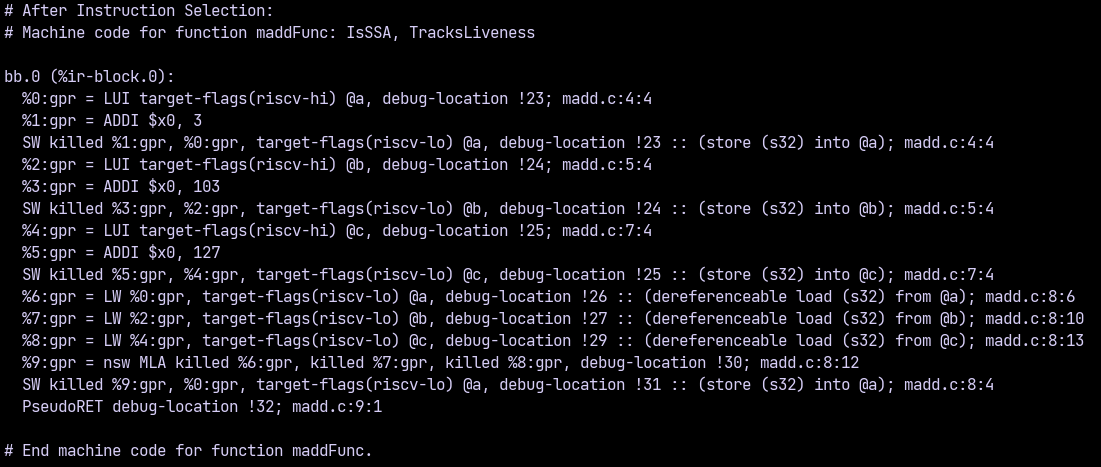
\includegraphics[width=0.9\textwidth]{path_instruction/madd_MachineInstruction.png}
    \caption{Machine Instruction before Register Allocation}
    \label{fig:mc_inst}
\end{figure}

\clearpage
\section{Machine Code Instruction}
After register allocation, Machine Code Instruction (MCInst) representation of the code is created. MCInst can be thought of as an intermediate representation of the lower-level code. It can be used to produce both an object file and an Assembly file. The generated Assembly is presented below:
\begin{lstlisting}[ caption=madd.s Assembly Output]
    maddFunc:                               # @maddFunc
# %bb.0:
	addi	sp, sp, -16
.Ltmp0:
	sw	ra, 12(sp)                      # 4-byte Folded Spill
	sw	s0, 8(sp)                       # 4-byte Folded Spill
	addi	s0, sp, 16
	lui	a0, %hi(a)
	li	a1, 3
	sw	a1, %lo(a)(a0)
	lui	a1, %hi(b)
	li	a2, 103
	sw	a2, %lo(b)(a1)
	lui	a2, %hi(c)
	li	a3, 127
	sw	a3, %lo(c)(a2)
	lw	a3, %lo(a)(a0)
	lw	a1, %lo(b)(a1)
	lw	a2, %lo(c)(a2)
	mla	a1, a3, a1 ,a2
	sw	a1, %lo(a)(a0)
	lw	ra, 12(sp)                      # 4-byte Folded Reload
	lw	s0, 8(sp)                       # 4-byte Folded Reload
	addi	sp, sp, 16
	ret
\end{lstlisting}